\documentclass[12pt]{amsart}
\usepackage{amsaddr}
\usepackage{marktext} 
%% Remove draft for real article, put twocolumn for two columns
\usepackage{svmacro}
\usepackage[utf8]{inputenc}
\usepackage{lineno}
\usepackage[style=alphabetic, backend=biber]{biblatex}
\addbibresource{bibliography.bib}

%% commentary bubble
\newcommand{\SV}[2][]{\sidenote[colback=green!10]{\textbf{SV\xspace #1:} #2}}

%% Title 
\title{ MATH 104: Worksheet 10}
\author{}

%\author{Co-author}
%\address{  }
%\email {  }
%
\date{03/04/2024}

\begin{document}


\maketitle


\section{Concepts}

\begin{enumerate}
	\item Partial derivative
	      \begin{equation*}
		      \partial_x f (x,y,z) = f_x (x,y,z) =
		      \lim_{h\to 0} \frac{ f(x+h, y,z) - f(x,y,z) }{h}
	      \end{equation*}
	      \begin{equation*}
		      \partial_y f (x,y,z) = f_y (x,y,z) =
		      \lim_{h\to 0} \frac{ f(x, y+h,z) - f(x,y,z) }{h}
	      \end{equation*}
	      \begin{equation*}
		      \partial_z f (x,y,z) = f_z (x,y,z) =
		      \lim_{h\to 0} \frac{ f(x, y, z+ h) - f(x,y, z) }{h}
	      \end{equation*}
	\item Gradient
	      \begin{equation*}
		      \grad f(x,y,z) = \langle f_x (x,y,z), f_y (x,y,z), f_z  (x,y,z)\rangle \,.
	      \end{equation*}
\end{enumerate}


\section{Discussions}

\begin{question}
	Find all partial derivatives of
	\begin{enumerate}
		\item  $$ f(x,y) = 3x^3 - 2x^2y^5$$
		      \vspace{7cm}
		\item  $$ f(x,y) = \frac{xy^2}{x+1} $$
		      \vspace{7cm}
		\item  \[ g(r,s) = rs \cos(r) \]
		      \vspace{7cm}
		\item  \[ f(w,x,y) = (6w+1) \cos(3x^2 + 4xy^3 + y) \]
		      \vspace{7cm}
		\item
		      \[
			      q(x,t,z) = \frac{x 2^t z^3}{1 + x^2}.
		      \]
		      \vspace{7cm}
	\end{enumerate}
\end{question}

\begin{question}
	Consider the following picture
	\begin{figure}[ht]
		\begin{center}
			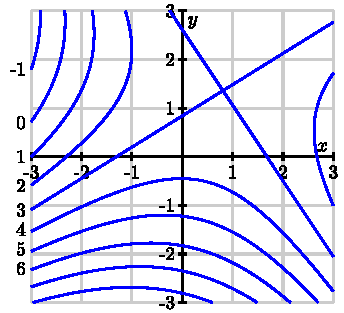
\includegraphics[width=0.8\textwidth]{fig/worksheet10-contour.pdf}
		\end{center}
	\end{figure}

	\begin{enumerate}
		\item Estimate the partial derivative \( f_x(-2, -1) \). (Hint: How can values of \( f \) that are of the form \( f(-2 + h) \) and \( f(-2 - h) \) be used to compute a symmetric difference quotient?)
		      \vspace{4cm}
		\item Estimate the partial derivative \( f_y(-2, -1) \).
		      \vspace{4cm}
		\item Estimate the partial derivatives \( f_x(-1,2) \) and \( f_y(-1,2) \).
		      \vspace{4cm}
		\item Locate, if possible, one point \( (x,y) \) where \( f_x(x,y) = 0 \).
		      \vspace{4cm}
		\item Locate, if possible, one point \( (x,y) \) where \( f_x(x,y) < 0 \).
		      \vspace{4cm}
		\item Locate, if possible, one point \( (x,y) \) where \( f_y(x,y) > 0 \).
		      \vspace{4cm}
	\end{enumerate}


\end{question}

\end{document}
